\documentclass[12pt]{book}

\usepackage[utf8]{inputenc}
\usepackage[T1]{fontenc}
\usepackage{geometry}
\usepackage{graphicx}
\usepackage[spanish]{babel}
\usepackage{amsthm}
\usepackage{amsmath}
\usepackage{trfsigns}

\newtheorem{thm}{Teorema}[section]
\theoremstyle{definition}
\newtheorem{dfn}{Definición}[section]
\theoremstyle{remark}
\newtheorem{note}{Nota}[section]
\theoremstyle{plain}
\newtheorem{lem}[thm]{Lema}

\geometry{letterpaper}



\title{Introducción al Diseño de Filtros Electrónicos}
\author{Dr. Casimiro Gómez González\\
	Facultad de Electrónica, UPAEP\\
               correo: casimiro.gomez@upaep.mx\\
               Tel: 222 229 9428}
\date{Primavera 2010}

\begin{document}
\frontmatter
\maketitle


\chapter{Prólogo}

El presente libro está diseñado para ser impartido en un semestre en las licenciatura en ingeniería Mecatrónica, Electrónica o Biónica. El material ha sido desarrollado a lo largo de varios años de experiencia impartiendo la materia en la Universidad Popular Autónoma del Estado de Puebla (UPAEP) en Puebla, México.

El material está auto contenido, es decir, se ha procurado que leyendo secuencialmente el libro se podrá diseñar filtros electrónicos analógicos al terminar de leerlo. Como podrá notarse, algunas partes del documento aún no se han terminado. Por lo cual el autor agradecerá cualquier sugerencia, comentario o correcciones que deseen realizar al presente documento. Como todo libro que se presuma de ser moderno se utilizan dos distintos software para el diseño y simulación de los filtros; en el aspecto del cálculo matemático se utiliza Maxima (http://maxima.sourceforge.net/es/)  y en la simulación electrónica se utiliza Multisim de National Instrument.

El material del libro esta organizado en seis capítulos en donde el primer capitulo es una breve introducción a la teoría de amplificadores, este material es necesario debido a que la técnica utilizada para el diseño de los filtros es la de amplificadores en cascada. Por lo que el estudiante debe manejar el diseño de amplificadores en cascada. Básicamente se da una introducción a los amplificadores operacionales bajo esta perspectiva.


\begin{flushright}

El autor\\
Casimiro Gómez González\\
Doctor en Ingeniería Mecatrónica
\end{flushright}

\tableofcontents

\mainmatter
\chapter{Diseño de Amplificadores}
Las señales de salida de los transductores son débiles (dentro el rango de los microvolts $\mu V$ y los milivolts $mV$) y poseen una cantidad de energía muy pequeña. El procesamiento de las señales es mucho más fácil si la magnitud de la señal es grande (en el rango de los volts). Un amplificador está compuesto por uno o más dispositivos amplificadores y su complejidad dependen del número de dispositivos de amplificación. Los objetivos del presente capitulo son:

\begin{itemize}
\item Familiarizarse con las características, los tipos, los modelos de circuito y las aplicaciones de los amplificadores
\item Aprender a definir las características de diseño de un amplificador para que cumpla los requerimientos de entrada y salida de una aplicación en particular
\item Familiarizarse con el teorema de Miller y sus aplicaciones para el análisis de amplificaciones realimentados.
\end{itemize}

\section{Características de un amplificador}
El amplificador puede ser considerado como una red de dos puertos, uno de entrada y uno de salida. Se representa por medio de un símbolo del circuito mostrado en la Figura \ref{fig1}, el cual indica la dirección del flujo de la señal, del lado de la entrada al lado de la salida. Por lo común una de las terminales de entrada se conecta a una de las terminales de salida para formar una tierra común. El voltaje (o corriente) de salida esta relacionado con el voltaje (o corriente) de entrada mediante un parámetro de ganancia.

\begin{figure}
\centering
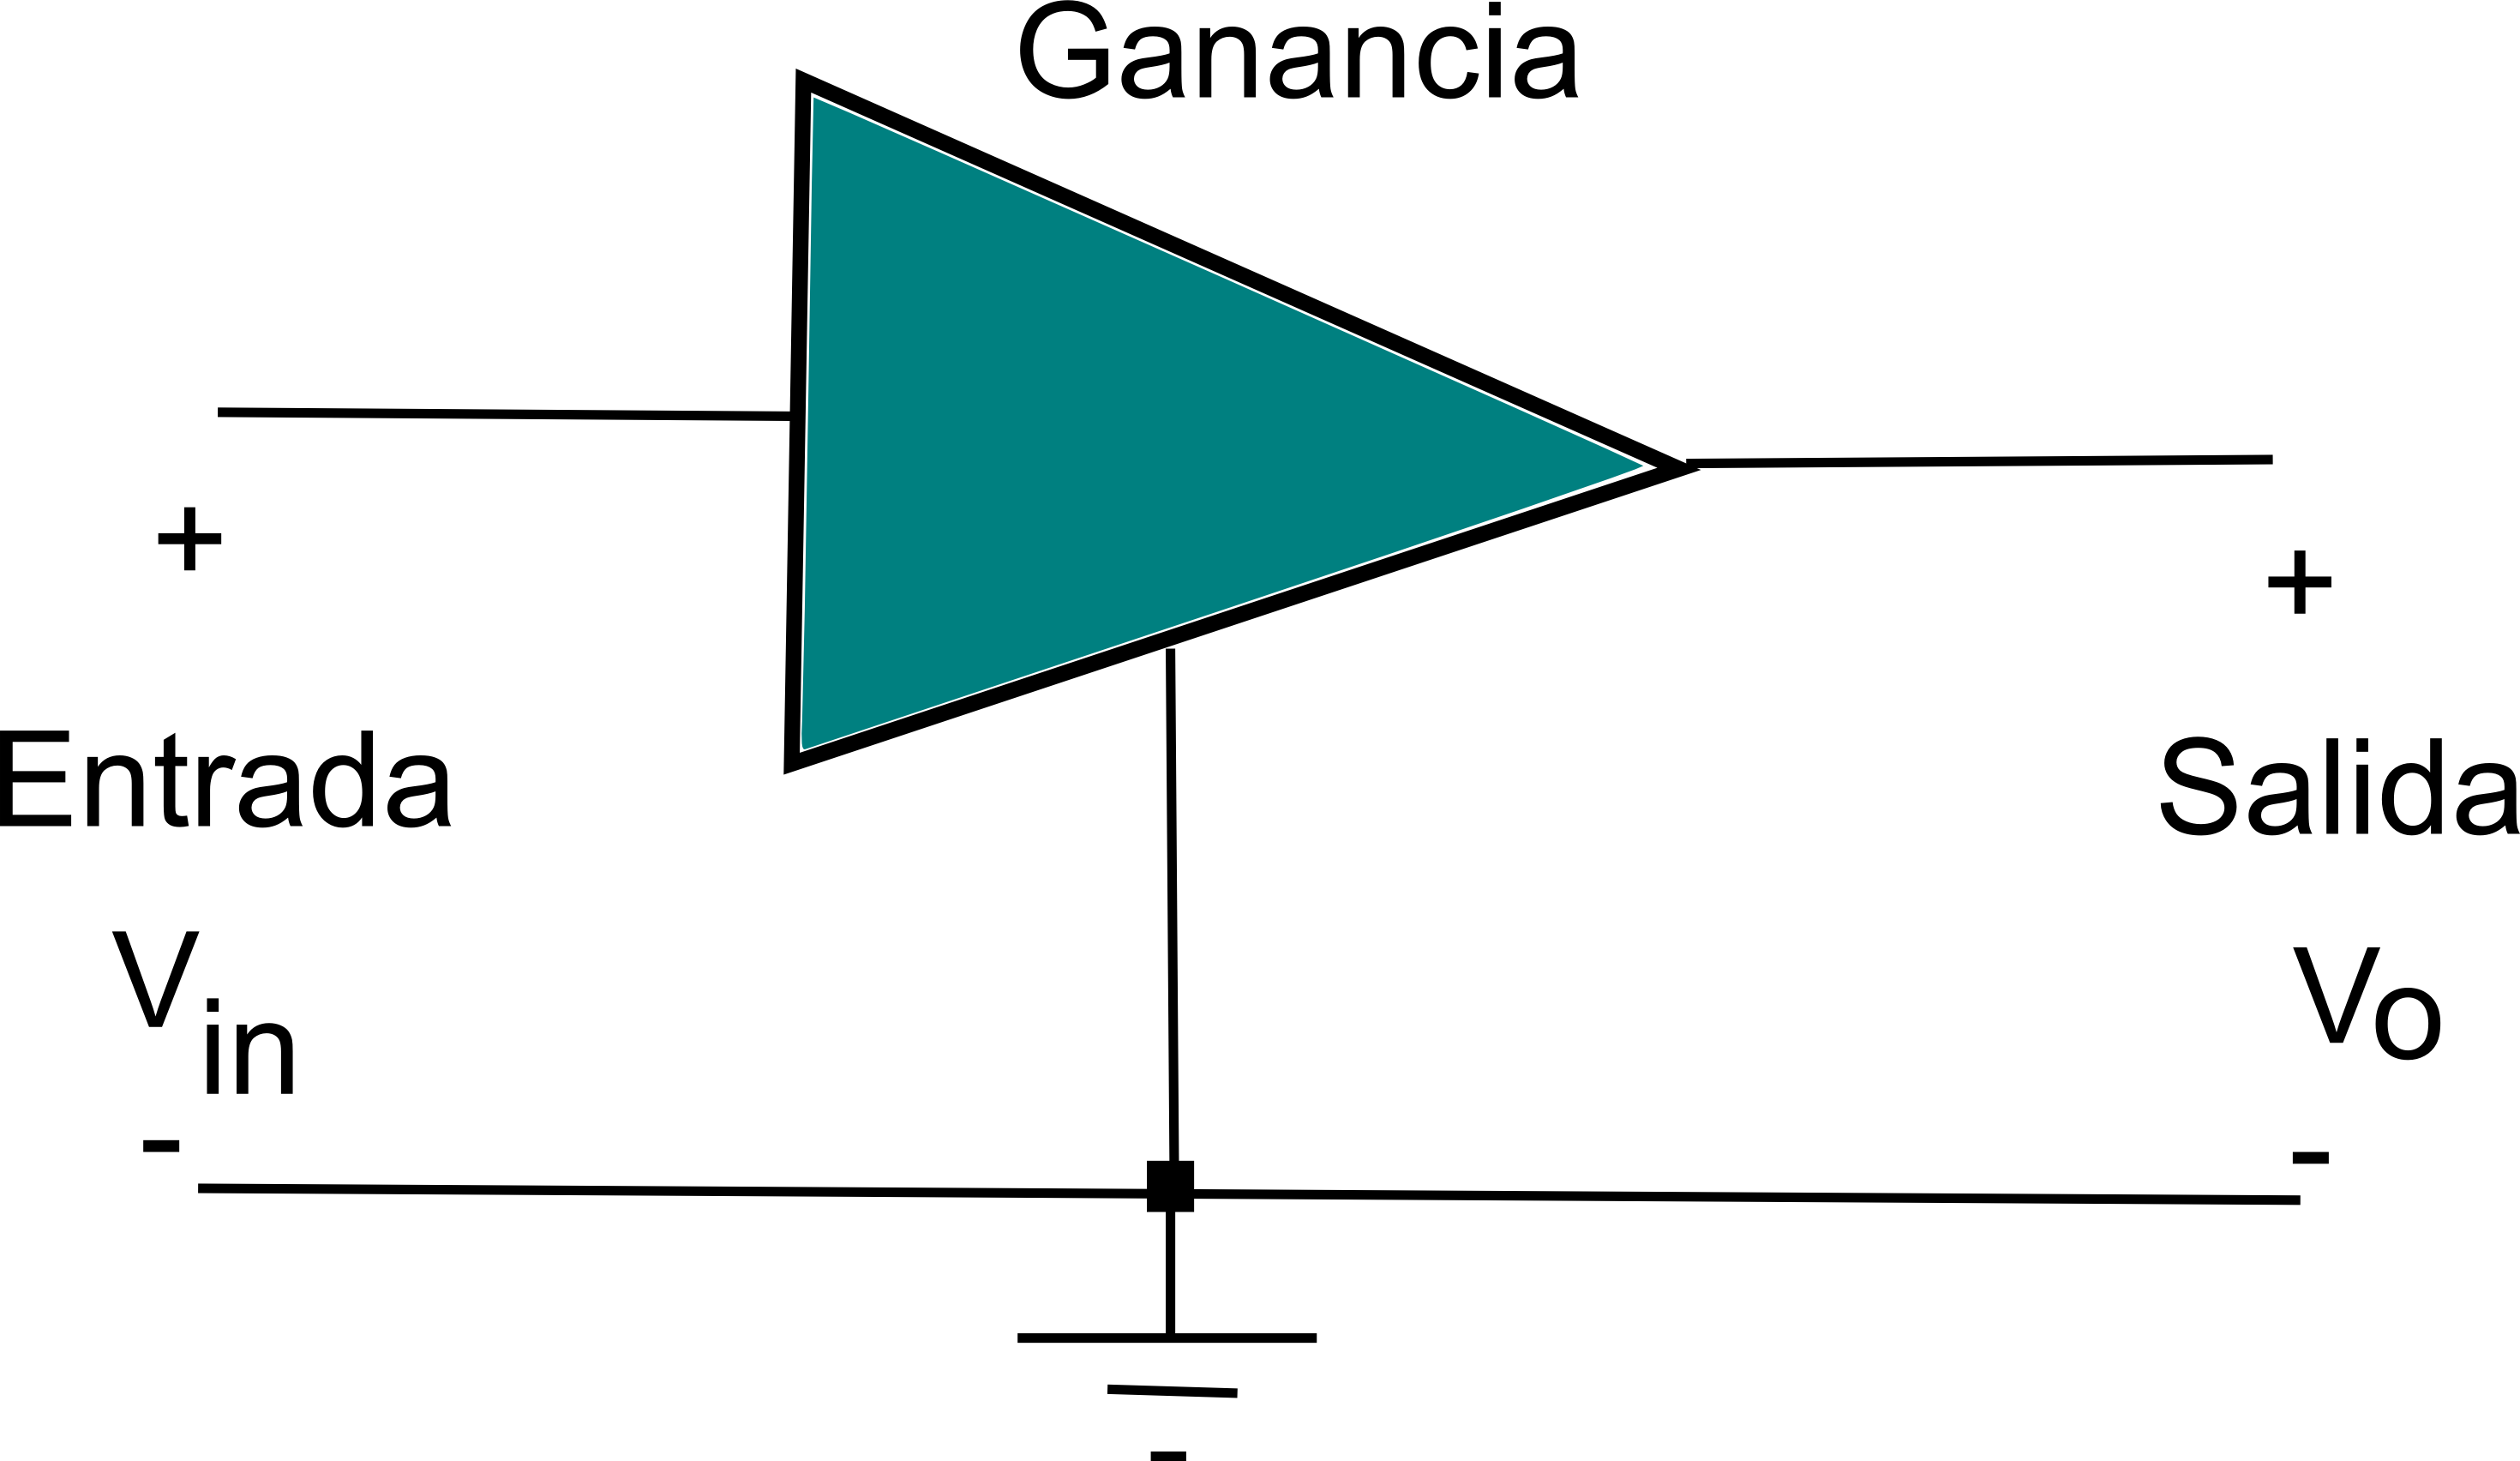
\includegraphics[width=3in]{Amplificador.png}
\caption{Símbolo de un amplificador}
\label{fig1}
\end{figure}

Si la señal de salida es directamente proporcional a la señal de entrada, de tal modo que sea un replica exacta de la señal de entrada, se dice que el amplificador es un amplificador lineal. Si cambia la onda de salida se considera que produce una distorsión, lo cual es indeseable entonces el amplificador es no lineal.

\subsection{Ganancia de voltaje}
Si el voltaje de entrada a un amplificador lineal es  $v_1$, entonces el amplificador produce un voltaje de salida $v_O$ , el cual es una réplica amplificada de  $v_1$. La ganancia de voltaje del amplificador  $A_v$ se define como:

 
\begin{dfn}
\label{def1}
Un amplificador lineal tiene una ganancia de voltaje $A_v$, la cual se define como:
$
A_v=\frac{v_O}{v_1}
$,
en donde $v_O$ es el voltaje de salida y $v_i$ el voltaje de entrada del amplificador
\end{dfn}

En el circuito de la figura \ref{fig2} podemos distinguir dos tipos de señales: La de corriente directa y la de corriente alterna. De aquí podemos decir que la ganancia de corriente directa es $A_v=\frac{V_O}{V_1}$, y sin embargo como esta superpuesta una señal de corriente alterna de la forma $v_i=V_m sen(\omega t)$ el voltaje de salida llega a ser $v_O=V_O+v_o$. La ganancia de voltaje de corriente alterna es $A_v=\frac{v_o}{v_i}$. Por lo tanto, un voltaje de entrada de la señal pequeña $v_i$ produce un voltaje de salida de señal pequeña correspondiente $v_O=A_v V_m sen(\omega t)$, tal que $v_O=V_O+A_v v_i=V_O+A_v V_m sen (\omega t)$.Si el amplificador es lineal entonces $A_V=A_v$.

\begin{figure}
\centering
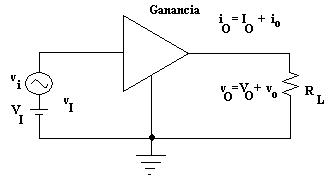
\includegraphics[width=3in]{Pequena.jpg}
\caption{Señal pequeña superpuesta sobre la señal de corriente directa}
\label{fig2}
\end{figure}

En la figura \ref{fig3}  se muestra el voltaje de salida de un amplificador lineal, como se puede observar la señal no se deforma tan solo se amplifica por un factor constante

\begin{figure}
\centering
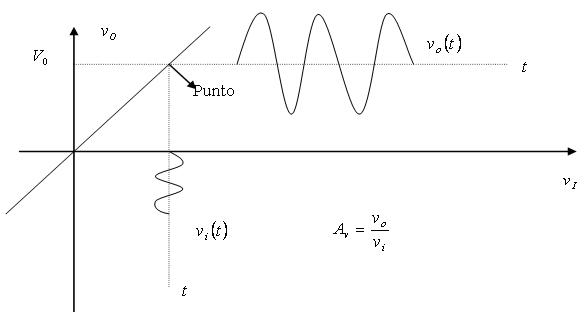
\includegraphics[width=3in]{VoltajeSalida.jpg}
\caption{Voltaje de salida de pequeña señal de un amplificador lineal}
\label{fig3}
\end{figure}

\subsection{Ganancia de corriente}
Si  $i_I$ es la corriente que el amplificador extrae de la fuente de señal, e   $i_O$ es la corriente que el amplificador entrega a la carga $R_L$ , entonces la ganancia de corriente   del amplificador la podemos definir de la siguiente forma:

\begin{dfn}
\label{def2}
Un amplificador lineal tiene una ganancia de corriente $A_I$, la cual se define como:
$
A_I=\frac{i_O}{i_I}
$,
en donde $i_O$ es la corriente de salida y $i_I$ es la corriente de entrada del amplificador
\end{dfn}

Para un amplificador lineal, la ganancia de corriente directa es igual a la ganancia de pequeña señal:  $A_I=A_i$  por lo que a la ganancia de pequeña señal se le conoce como ganancia de corriente.

\subsection{Ganancia de Potencia}

Un amplificador proporciona a la carga una mayor potencia que la que recibe de la fuente de señal. Por lo tanto, el amplificador tiene una ganancia de potencia  $A_p$  definida por

\begin{dfn}
\label{def3}
Un amplificador lineal tiene una ganancia de potencia $A_p$, la cual se define como:
$
A_p=\frac{P_L}{P_I} =\frac{v_O i_O}{v_I i_I}=A_v A_i
$,
en donde $P_O$ es la potencia de salida y $P_I$ es la potencia de entrada del amplificador lineal
\end{dfn}

\subsection{Ganancia logarítmica}
Las ganancias de los amplificadores pueden expresarse como cantidades dimensionales o con unidades ($V/V$  para ganancias en voltaje, $A/A$ para ganancias es corriente o $W/W$ para ganancias en potencia). Por lo general, sus valores son muy grandes y abarcan varios órdenes de magnitud. Es común que las ganancias se expresen en términos de logaritmos conocidos como decibeles, en el caso de la ganancia de voltaje expresada en decibeles la expresión es $A_{dB}=20 \log \mid A_v \mid$.
La ganancia de potencia se calcula utilizando las siguientes ecuaciones:

$A_{dB}=10 \log (A_p)=10 \log (\frac{P_L}{P_i})=10 \log (\frac{\frac{v^2_o}{R_L}}{\frac{v^2_i}{R_i}})=20 \log (\frac{v_o}{v_i})+10 \log (\frac{R_i}{R_L})$

En donde $R_i$  es la resistencia de entrada del amplificador y $R_L$  es la resistencia de carga. El término $20 \log (\frac{v_o}{v_i})$  se conoce como ganancia en voltaje del amplificador. Si tenemos el caso de que la resistencia de entrada y la resistencia de salida del amplificador sean iguales, es decir, $R_L=R_i$ entonces:

$A{p,dB}=20 \log (A_v)$

La ganancia de potencia en dB también se puede dejar en función de las corrientes de entrada y de salida:
 
$A_{dB}=10 \log (A_p)=10 \log (\frac{P_L}{P_i})=10 \log (\frac{i^2_o R_L}{i^2_i R_i})=20 \log (\frac{i_o}{i_i})+10 \log (\frac{R_i}{R_L})$

En donde $R_i$  es la resistencia de entrada del amplificador y $R_L$  es la resistencia de carga. El término $20 \log (\frac{i_o}{i_i})$  se conoce como ganancia en corriente del amplificador. Si tenemos el caso de que la resistencia de entrada y la resistencia de salida del amplificador sean iguales, es decir, $R_L=R_i$ entonces:

$A{p,dB}=20 \log (A_i)$

\subsection{Resistencia de entrada y de salida }
La resistencia de entrada  es una medida de la corriente extraída por el amplificador. Es la razón del voltaje de entrada entre la corriente de entrada

\begin{equation}
\label{equ7}
R_I=\frac{v_I}{i_I}
\end{equation}

La resistencia de salida  $R_O$  es la resistencia interna vista desde las terminales de salida de un amplificador; es decir, la resistencia equivalente de Thévenin. Su definición es

\begin{equation}
\label{equ8}
R_O=\frac{v_O}{i_O}
\end{equation}

\section{Tipos de amplificadores}

La señal de entrada de un amplificador puede ser una fuente de voltaje o una fuente de corriente. La salida de un amplificador puede ser una fuente de voltaje o una fuente de corriente. Por tanto, existen cuatro posibles combinaciones de entrada y salida: $v-v$, $i-i$ , $v-i$ , e  $i-v$. Con base en las relaciones de entrada y de salida, los amplificadores se clasifican en: amplificadores de voltaje, amplificadores de corriente, amplificadores de transconductancia y amplificadores de transimpedancia.

\subsection{Amplificador de voltaje}

Un amplificador cuyo voltaje de salida es proporcional a su voltaje de entrada se conoce como amplificador de voltaje. La señal de entrada es una fuente de voltaje; la salida del amplificador también es una fuente de voltaje. Este amplificador se conoce como una fuente de voltaje controlada por voltaje (FVCV).En la figura \ref{fig4} se muestra un ejemplo. El amplificador esta conectado entre una fuente de voltaje $v_s$ y una resistencia de carga $R_L$. $R_s$ es la resistencia de la fuente.  $A_{vo}$  es la ganancia de voltaje con la resistencia de carga $R_L$ desconectada, y se conoce como ganancia en voltaje a circuito abierto. $R_0$ es la resistencia de salida del amplificador. Además de amplificar una señal de voltaje, el amplificador de voltaje puede tener otros usos, como simular una resistencia negativa o multiplicar la capacitancia.


\begin{figure}
\centering
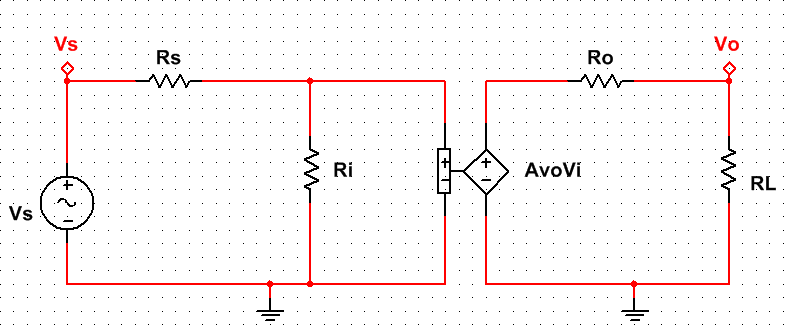
\includegraphics[width=3.5in]{AmplificadorVoltaje.png}
\caption{Circuito equivalente de señal pequeña de una Amplificador de Voltaje}
\label{fig4}
\end{figure}

En la figura \ref{fig5} se muestra los voltaje de entrada y salida de un amplificador de voltaje. Como podrá notarse la señal del voltaje de salida es mayor al voltaje de entrada. Ambas señales en este ejemplo están en fase.
\begin{figure}
\centering
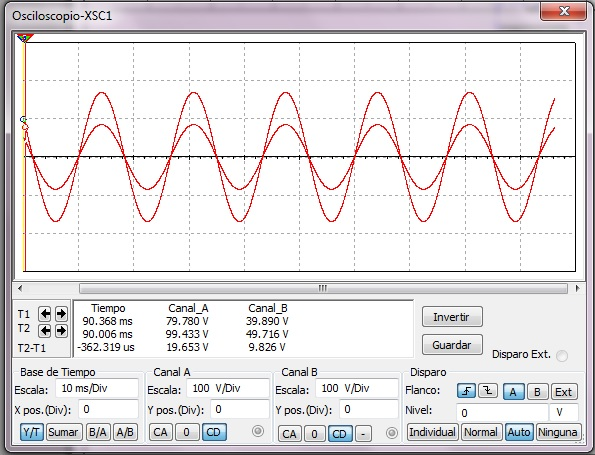
\includegraphics[width=3.5in]{senalamplificador.jpg}
\caption{Señales de voltaje del amplificador}
\label{fig5}
\end{figure}

El voltaje de salida de un amplificador de voltaje se obtiene por medio de la regla del divisor de voltaje

\begin{equation}
\label{equ9}
v_0 = i_0 R_L = A_{v0} v_i \frac{R_L}{R_L+R_0}
\end{equation}

De acuerdo con esta regla, el voltaje de entrada al amplificador $v_i$ esta relacionada con el voltaje de la señal $v_s$ por
\begin{equation}
\label{equ10}
v_i = \frac{R_i}{R_i+R_s} v_s
\end{equation}

Sustituyendo $v_i$ de la ecuación \ref{equ10} en la ecuación \ref{equ9}, se obtiene la ganancia en voltaje efectiva $A_v$, la cual se define como la relación $v_0$ respecto de $v_s$, esto

 \begin{equation}
\label{equ11}
A_v= \frac{v_0}{v_s} = \frac{v_0}{v_i} \frac{v_i}{v_s}= A_{v0} \frac{R_i}{R_i+R_s} \frac{R_L}{R_L+R_0}
\end{equation}

La ganancia de corriente $A_i$, la cual se define como la relación de la corriente de salida $i_0$ respecto de la corriente de entrada $i_s$ ($=i_i$), esta dada por

\begin{equation}
\label{equ12}
A_i= \frac{i_0}{i_s} = \frac{A_{v 0} v_i}{R_L+R_0} \frac{1}{\frac{v_i}{R_i}}=\frac{A_{v 0} R_i}{R_L+R_0}
\end{equation}

La ganancia en potencia es el producto de la ganancia en voltaje por la ganacia en corriente. Es decir,
\begin{equation}
\label{equ13}
A_p = A_v A_i
\end{equation}

\subsection{Amplificador de corriente}

Un amplificador cuya corriente de salida es proporcional a su corriente de entrada, se conoce como amplificador de corriente. Su entrada es una fuente de corriente y su salida es una resistencia de carga $R_L$. Un amplificador de corriente se representa por medio de una fuente de corriente controlada por corriente (FCCC), como se muestra en la figura \ref{fig6}. $A_{i s}$ se denomina ganancia en corriente en cortocircuito ( o simplemente ganancia de corriente) con las terminales de salida puestas en cortocircuito. $R_i$ es la resistencia de entrada y $R_0$ es la resistencia de salida. Es común utilizar el amplificador de corriente para proporcionar una ganancia en voltaje modesta, pero con una importante ganancia de corriente, de modo que este absorba poca potencia de la fuente de señal y entregue una gran cantidad de potencia a la carga. Este tipo de amplificador a menudo se conoce como amplificador de potencia.

\begin{figure}
\centering
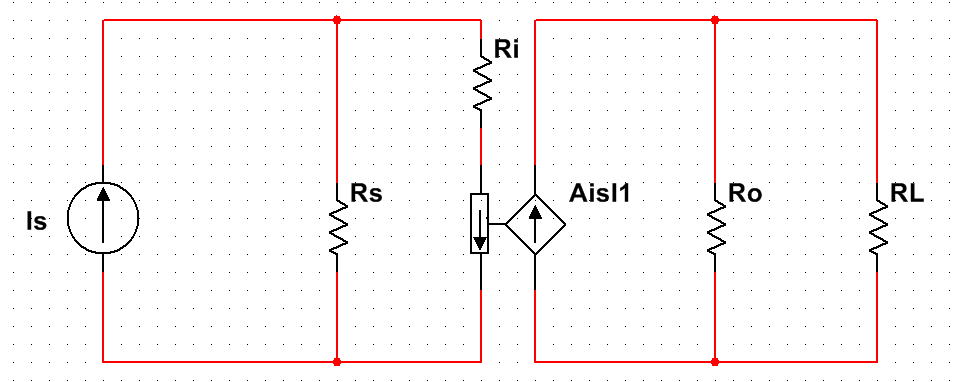
\includegraphics[width=4in]{amplificadorcorriente.png}
\caption{Amplificador de Corriente}
\label{fig6}
\end{figure}

La corriente de salida del amplificador se obtiene con la regla del divisor de corriente

\begin{equation}
\label{equ14}
i_0 = A_{i s} i_i \frac{R_0}{R_0+R_L}
\end{equation}

La corriente de entrada $i_i$ del amplificador esta relacionada con la corriente de la fuente de señal $i_s$ por
\begin{equation}
\label{equ15}
i_i =  i_s \frac{R_s}{R_s+R_i}
\end{equation}

Sustituyendo $i_i$ de la ecuación de la ecuación \ref{equ15} en la ecuación \ref{equ14}, se obtiene la ganancia de corriente efectiva $A_i$, la cual se define como la relación de $i_0$ respecto de $i_s$. Es decir,

\begin{equation}
\label{equ16}
A_i = \frac{i_0}{i_s} = \frac{i_0}{i_i} \frac{i_i}{i_s}= A_{i s} \frac{R_s}{R_s+R_i} \frac{R_0}{R_0+R_L}
\end{equation}

La ganancia en voltaje $A_v$, la cual se define como la relación del voltaje de salida $v_0$ respecto del voltaje de entrada $v_s$, esta dada por

\begin{equation}
\label{equ17}
A_v = \frac{v_0}{v_s}=A_i \frac{R_L}{R_s}
\end{equation}

La ganancia en potencia es el producto de la ganancia en voltaje por la ganancia en corriente. Esto es,
\begin{equation}
\label{equ18}
A_p = A_v A_i
\end{equation}

\subsection{Amplificadores de transconductancia}

Una amplificador que recibe una señal de voltaje como entrada y que proporciona una señal de corriente como salida se llama amplificador de transconductancia; en la figura \ref{fig7} se muestra un ejemplo. puede representarse por medio de una fuente de corriente controlada por voltaje (FCCV). El amplificador se conecta entre una fuente de voltaje $v_s$ y una resistencia de carga $R_L$. El parámetro de ganancia $G_{m s}$, que es la relación de la corriente de salida en cortocircuito respecto al voltaje de entrada, se llama transconductancia en cortocircuito. De acuerdo con la regla del divisor de corriente, la corriente de salida $i_0$ es
\begin{equation}
\label{equ19}
i_0 = G_{m s} v_i \frac{R_0}{R_0+R_L}
\end{equation}
El voltaje de entrada $v_i$ del amplificador está relacionado con la fuente de voltaje $v_s$ por

\begin{equation}
\label{equ20}
v_i = \frac{R_i}{R_i+R_s} v_s
\end{equation}

\begin{figure}
\centering
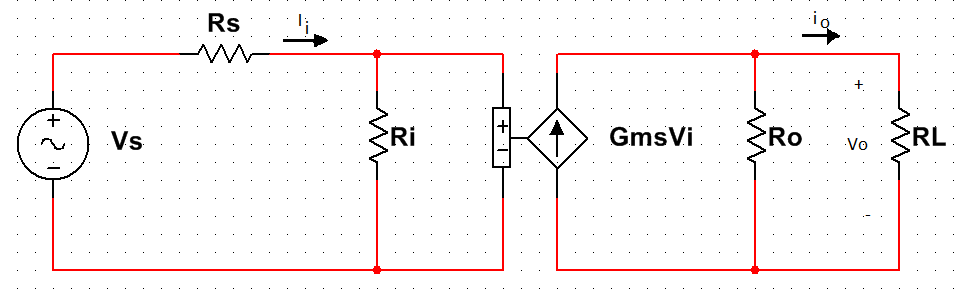
\includegraphics[width=4in]{amplificadortransconductancia.png}
\caption{Amplificador de Transconductancia}
\label{fig7}
\end{figure}

Sustituyendo $v_i$ de la ecuación \ref{equ20} en la ecuación \ref{equ19} se obtiene la ganancia en transconductancia efectiva $G_m$ como

\begin{equation}
\label{equ21}
G_m = \frac{i_0}{v_s}= G_{m s} \frac{R_0}{R_0+R_L} \frac{R_i}{R_i+R_s}
\end{equation}

La ganancia en voltaje efectiva $A_v$ es

\begin{equation}
\label{equ22}
A_v = \frac{v_0}{v_s}=\frac{v_0}{v_i} \frac{v_i}{v_s}= G_{m s} \frac{R_0 R_L R_i}{(R_0+R_L)(R_i+R_s)}
\end{equation}

\subsection{Amplificadores de transimpedancia}
La señal de entrada a un amplificador de transimpedancia es una fuente de corriente, y su salida es una fuente de voltaje. Éste puede representarse por una fuente de voltaje controlada por corriente (FVCC), como se muestra en la figura \ref{fig7} El parámetro de ganancia $Z_{m 0}$ es la relación del voltaje de salida del circuito abierto respecto a la corriente de entrada, y se denomina transimpedancia a circuito abierto (o simplemente transimpedancia).


\begin{figure}
\centering
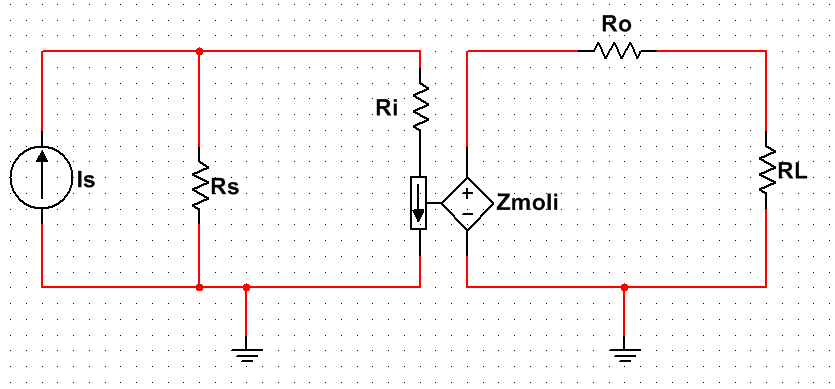
\includegraphics[width=4in]{AmplificadoresTransImpedancia.png}
\caption{Amplificador de TransImpedancia}
\label{fig8}
\end{figure}

El voltaje de salida $v_0$ está relacionado con $i_i$ como se indica a continuación:

\begin{equation}
\label{equ23}
v_0 = Z_{m 0} i_i \frac{R_L}{R_L+R_0}
\end{equation}

La corriente de entrada $i_i$ del amplificador está relacionada con $i_s$ de la siguiente manera:

\begin{equation}
\label{equ24}
i_i = \frac{R_s}{R_s+R_i} i_s
\end{equation}

Sustituyendo $i_i$ de la ecuación \ref{equ24} en la ecuación \ref{equ23}, se obtiene la transimpedancia efectiva $Z_m$

\begin{equation}
\label{equ25}
Z_m = \frac{v_0}{i_s}= Z_{m 0} \frac{R_L}{R_L+R_0} \frac{R_s}{R_s+R_i}
\end{equation}


La ganancia en voltaje efectiva $A_v$ es

\begin{equation}
\label{equ26}
A_v = \frac{v_0}{v_s} = Z_{m 0} \frac{1}{R_s+R_i} \frac{R_L}{R_L+R_0}
\end{equation}

\section{Teorema de Miller}

El teorema de Miller simplifica el análisis de los amplificadores retroalimentados. El teorema establece que si se conecta una impedancia entre las terminales de entrada y salida de un amplificador de voltaje, esta impedancia puede ser remplazada por dos impedancias equivalentes: una conectada a través de la entrada y la otra a través de las terminales de salida. 

\begin{figure}
\centering
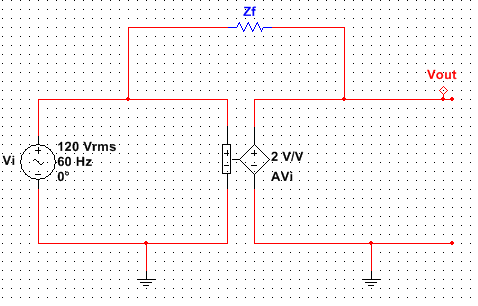
\includegraphics[width=4in]{AmplificadorMiller.png}
\caption{Amplificador retroalimentado}
\label{fig1000}
\end{figure}

\begin{figure}
\centering
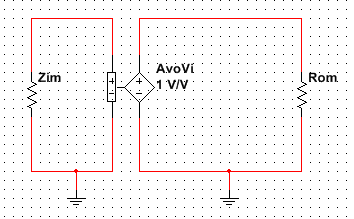
\includegraphics[width=4in]{EquivalenteMiller.png}
\caption{Equivalente de Miller}
\label{fig1001}
\end{figure}

En las figuras \ref{fig1000} y \ref{fig1001} se muestra la relación que existe entre el amplificador y su circuitos equivalente. Con la selección de los valores apropiados de las impedancias $Z_{im}$ y $Z_{om}$, el comportamiento de los circuitos de las figuras \ref{fig1000} y \ref{fig1001} puede hacerse idéntico. 

Si $A_{v0}$ es la ganancia en voltaje a circuito abierto del amplificador, el voltaje de salida $V_0$ está relacionado con el voltaje de entrada $V_i$ por


\begin{equation}
\label{equ1000}
V_0=A_{vo} V_i
\end{equation}

La corriente de entrada $I_i$ del amplificador de la figura \ref{fig1000} es
\begin{equation}
\label{equ1001}
I_{i}=\frac{V_{i}-V_{0}}{Z_{f}}
\end{equation}

La sustitución de $V_{0}$ de la ecuación \ref{equ1001} en la \ref{equ1000} da

\begin{equation}
\label{equ1002}
I_{i}=\frac{V_{i}-A_{v0}V_{i}}{Z_{f}}=V_{i}(\frac{1-A_{v0}}{Z_{f}})
\end{equation}

La impedancia de entrada $Z_{i}$ del circuito de la figura \ref{fig1001} debe ser igual a la del circuito de la figura \ref{fig1000}, y se calcula con la ecuación \ref{equ1002}:

\begin{equation}
\label{equ1003}
Z_{im}=\frac{V_{i}}{I_{i}}=\frac{Z_{f}}{1-A_{vo}}
\end{equation}

La corriente de salida $I_{o}$ del circuito de la figura \ref{fig1000} es
\begin{equation}
\label{equ1004}
I_{o}=\frac{V_{o}-V_{i}}{Z_{f}}
\end{equation}
Sustituyendo $V_{i}$ de la ecuación \ref{equ1001} en la \ref{equ1004}, se obtiene

\begin{equation}
\label{equ1005}
I_{o}=\frac{V_{o}-V_{o}/A_{vo}}{Z_{f}}=V_{o}(\frac{1-1/A_{vo}}{Z_{f}})
\end{equation}

La impedancia de salida $Z_{om}$ del circuito de la figura \ref{fig1001} debe ser igual a la del circuito de la figura \ref{fig1000}, y se calcula con la ecuación \ref{equ1005}:

\begin{equation}
\label{equ1006}
Z_{om}=\frac{V_{o}}{I_{o}}=\frac{Z_{f}}{1-1/A_{vo}}=\frac{Z_{f}A_{vo}}{A_{vo}-1}
\end{equation}

\section{Ejemplo: Utilización del teorema de Miller}

Se conecta un capacitor $C=0.01 \mu F$ a través de los lados de entrada y salida de un amplificador , como se muestra en la  figura \ref{fig1002}. Los parámetros del amplificador son $A_{vo}=-502$, $R_{o} =50 \Omega$ y $R_{i}=100 k \Omega$. La resistencia de la fuente es $R_{s}=2 k\Omega$ y la resistencia de la carga es $R_{L}=10 k\Omega$.

\begin{itemize}
\item (a) Usar el teorema de Miller para calcular la frecuencia de corte
\item Encontrar una expresión para la ganancia en función de la frecuencia 
\end{itemize}

\subsection{(a)}
Se tiene

\begin{equation}
A_{v}\approx \frac{R_{L}A_{vo}}{R_{L}+R_{o}}=\frac{(10k\Omega)(-502)}{10k\Omega+50\Omega}=-500
\label{equ1007}
\end{equation}

Si se reemplaza $C$ con su capacitancia de Miller, se obtiene el circuito equivalente de la figura \ref{fig1003}. Al sustituir $Z_{f}=1/j2\pi fC$ en la ecuación \ref{equ1003}, se obtiene

\begin{equation}
Z_{im}=\frac{1}{j2 \pi f C (1-A_{v})}=\frac{1}{j 2 \pi f C_{im}}
\label{equ1008}
\end{equation}


\begin{figure}
\centering
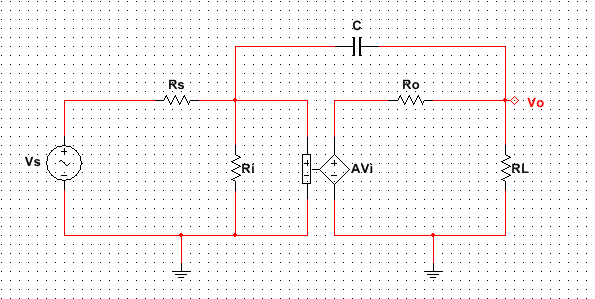
\includegraphics[width=4in]{ejemploMiller.png}
\caption{Ejemplo de Amplificador}
\label{fig1002}
\end{figure}

en donde la capacitancia de Miller $C_{im}$ a través de la entrada es

\begin{equation}
C_{im}=C(1-A_{v})=0.001 \mu F (1+500)=5.01 \mu F
\label{equ1009}
\end{equation}

\begin{figure}
\centering
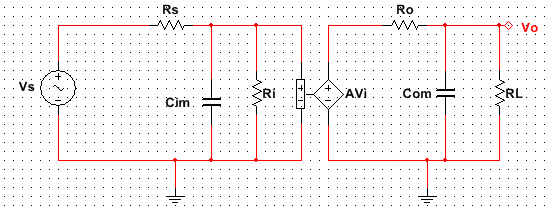
\includegraphics[width=4in]{SolucionEjemploMiller.png}
\caption{Solución del ejemplo de Miller}
\label{fig1003}
\end{figure}

Al sustituir $Z_{f}=1/j2 \pi f C$ en la ecuación \ref{equ1006}, se obtiene

\begin{equation}
Z_{om}=\frac{1}{j2 \pi f C (1-1/A_{v})}=\frac{1}{j 2 \pi f C_{om}}
\label{equ1010}
\end{equation}

de donde la capacitancia de Miller $C_{om}$ a través de la salida es

\begin{equation}
C_{om}=C(1-1/A_{v})=0.001 \mu F (1+1/500)=0.01 \mu F
\label{equ1011}
\end{equation}


La constante de tiempo $\tau _{1}$ para $C_{im}$ se obtiene por inspección, debido a que $C_{im}$ se descarga si la fuente $V_{s}$ se pone en cortocircuito) a través de la combinación en paralelo de $R_{s}$ y $R_{i}$. Esto es

\begin{equation}
\tau _{1}=C_{im}   (R_{s}\parallel R_{i})=5.01 \mu F (2K \parallel 100k)=9.824 ms
\label{equ1012}
\end{equation}

La primera frecuencia de corte es $\omega _{1}=1/ \tau _{1}=1/9.824 ms=101.8 rad/seg$

La constante de tiempo $\tau _{2}$ para $C_{om}$ también se obtiene por inspección ya que $C_{om}$ se descarga (si la fuente $V_{s}$ se pone en corto circuito) a través de la combinación en paralelo de $R_{o}$ y $R_{L}$. Esto es,

\begin{equation}
\tau _{2}=C_{om}(R_{L} \parallel R_{o})=0.01 \mu F (10\parallel 50)=0.498 \mu s
\label{equ1013}
\end{equation}

La segunda frecuencia de corte es $\omega _{2}=1/\tau _{2}$

\subsection{(b)}

La ganancia en función de la frecuencia $A_{v}(j\omega)$ es
\begin{equation}
A_{v}(j\omega)= \frac{V_{0}(j 0)}{V_{s}(j \omega)}
\label{equ1014}
\end{equation}


\section{Problemas para resolver}

\subsubsection{Problema de diseño 1}

Se requiere un amplificador para amplificar la señal de salida de un transductor que produce una señal de voltaje $v_s=10$ mV con una resistencia interna $R_s=2.5 k \Omega$. La resistencia de carga $R_L$ es variable y cambia desde $2 k \Omega$ hasta $10 k \Omega$. El voltaje de salida deseado es $v_0=5 $ V. El amplificador no debe consumir mas de $1 \mu A$ del transductor. La variación del voltaje de salida cuando se desconecta la carga no debe ser menor que $0.5\%$. Determine las especificaciones de diseño del amplificador

\subsubsection{Problema de diseño 2}

Se requiere un amplificador para producir una ganancia en voltaje $A_v =100 \pm 1.5 \%$. La resistencia de la fuente $R_s$ es variable, entre $500 \Omega$ y $5 k \Omega$, y la resistencia de carga $R_L$ cambia entre $5 k  \Omega$ y $20 k \Omega$. Determine las específicaciones de diseño del amplificador.

\subsubsection{Problema de diseño 3}

Se requiere un amplificador para amplificar la señal de salida de un transductor que produce una corriente constante $i_s = 100 \mu A$ con una resistencia interna variable desde $R_s=10 k \Omega$ hasta  $R_s=100 k \Omega$. La corriente de salida deseada es $i_0 = 20 mA$ con una resistencia de carga variable desde  $R_L=20 \Omega$ hasta  $R_L=500 \Omega$. La variación de la corriente de salida se debe mantener dentro $\pm 3 \%$. Determine las especificaciones de diseño del amplificador.


\subsubsection{Problema de diseño 4}

Se requiere un amplificador para producir una ganancia en corriente $A_i = 50 \pm 1.5 \%$. La resistencia de la fuente es $R_s=100 k \Omega$ y la resistencia de carga es $R_L= 100 \Omega$. Determine las especificaciones de diseño del amplificador.

\subsubsection{Problema de diseño 5}
Se requiere un amplificador para producir una ganancia de tramsconductancia $Z_m=20 mA/V \pm 2\% $. La resistencia de la fuente es $R_s = 1k \Omega$ y la resistencia de carga es $R_L=200 \Omega$. Determine las especificaciones de diseño del amplificador.

\section{Problemas para el examen de filtros electrónicos}

\subsection{Problema Grupo 1:}
Se requiere un amplificador para producir una ganancia en transconductancia $G_m = 20 mA/V \pm 2 \%$. La resistencia de la fuente es $R_s = 1 K \Omega $ y la resistencia de carga es $R_L = 200 \Omega$. Determine las especificaciones de diseño del amplificador

\subsection{Problema Grupo 2:}

Se requiere un amplificador para producir una ganancia en corriente $A_i = 50 \pm 1.5 \%$. La resistencia de la fuente es $R_s = 100 K \Omega$ y la resistencia de carga es $R_L= 100 \Omega$. Determine las especificaciones de diseño del amplificador.

\chapter{Introducción a la teoría de filtros}
Un filtro eléctrico  es un sistema eléctrico que puede ser usado para modificar, manipular y cambiar la forma del espectro de frecuencia de una señal eléctrica en base a un conjunto de requerimientos previos. Por ejemplo, un filtro puede ser usado para amplificar o atenuar un rango de componentes de frecuencias, rechazar o aislar una frecuencia específica entre otras. Las aplicaciones de los filtros son numerosas, por ejemplo,

\begin{itemize}
\item Para eliminar señales de ruido que contaminan los sistemas de comunicación
\item para separar señales relevante de irrelevantes
\item para detectar señales de radio y TV
\item para demodular señales
\item Para limitar en ancho de banda de señales antes de muestrearlas
\item Para convertir señales muestreadas en señales en tiempo continuo
\item para mejorar la calidad de las señales de audio, por ejemplo bocinas
\item Para la síntesis de voz
\item En la ecualización de las lineas de transmisión y cables
\item Para el diseño de implantes cocleares
\end{itemize}

Típicamente, un filtro eléctrico recibe una señal de entrada o exitación y produce una señal de salida o respuesta. El espectro de frecuencia de la señal de salida esta relacionada con la señal de entrada por medio de alguna regla de correspondencia. Dependiendo del tipo de entrada, salida o de las señales de operación internas, tres tipos generales de filtros pueden ser identificados, llamados, filtros de tiempo continuo, de datos muestreados o de tiempo discreto.

Una señal de tiempo continuo es una señal que esta definida en cada instante de tiempo. Y puede ser representada por una función $x(t)$ cuyo dominio se encuentra en el rango $(t_1,t_2)$, en donde $- \infty \leq t_1$ y $t_2 \leq \infty$.Una señal de datos muestreados o señal modulada en impulsos es una que es definida en términos de una suma infinita de impulsos de tiempo. Lo cual se puede representar por medio de la función

\begin{equation}
\label{equ27}
\widehat{x}(t) = \sum_{n= \infty}^{\infty} x(n T) \delta (t-n T)
\end{equation}

donde $\delta (t)$ es una función impulso. Los valores de la señal en cualquier instante del rango $n T<t <(n+1)T$ es cero. El espectro de frecuencia para una señal de tiempo continuo o una señal de muestreo de datos se obtiene por medio de la transformada de Fourier.
 Una señal de tiempo discreto esta definida en intervalos discretos de tiempo. Y puede estar representada por una función $x(n T)$, donde $T$ es una constante y $n$ es un entero en el rango $(n_1,n_2)$ tales que $- \infty \leq n_1$ y $n_2 \leq \infty$. El valor de la señal en cualquier instante dentro del rango $n T <t<(n+1) T$ puede ser cero, constante, o indefinido dependiendo de la aplicación. El espectro de frecuencia en este caso se obtiene evaluando la transformada $z$ en el círculo unitario $\mid z \mid=1$ del plano $z$.

Dependiendo del formato de las señales de entrada, salida y las operaciones internas, los filtros pueden ser clasificados en filtros analógicos y filtros digitales. En los filtros analógicos las señales de con las que se trabaja son voltajes y corrientes variables, mientras que en los filtros digitales las señales son codificadas en un formato binario. Los filtros de tiempo continuo y de muestreo de datos son siempre analógicos. Sin embargo, los filtros discretos pueden ser analógicos o digitales.

Los filtros analógicos pueden ser clasificados en base a los componentes que lo constituyen como

\begin{itemize}
\item Filtros pasivos RLC
\item Filtros de cristal
\item Filtros Mecánicos
\item Filtros de Microondas
\item Filtros Activos RC
\item Filtros de capacitores conmutados
\end{itemize}

Los filtros pasivos RLC estan formados por capacitores, inductores y resistencias. Los filtros de cristal esta formados por resonadores piezoeléctricos que pueden ser modelados por circuitos resonantes. Los filtros mecánicos estan hechos con resonadores mecánicos. Los filtros de Microondas estan formados por resonadores de microondas y cavidades que pueden ser representados por circuitos resonantes. Los filtros activos RC estan formados por resitencias, capacitores y amplificadores; en estos filtros, el comportamiento de los circuitos resonantes es simulado a través del uso de retroalimentaciones o por fuentes de energía para los circuitos pasivos. Los filtros de capacitores conmutados estan formados por resistencias, capacitores amplificadores e interruptores. Estos son filtros discretos en tiempo que funcionan como filtros activos pero a través de usar interruptores los valores de capacitancia se pueden mantener en valores muy pequeños. Como resultado los filtros de capacitores conmutados son viables de implementarse con tecnología VLSI.

\section{Caracterización}
Un filtro analógico lineal y causal con entrada $x(t)$ y salida $y(t)$ puede ser caracterizada por una ecuación diferencial de la forma

\begin{equation}
\label{equ28}
b_n \frac{d^n y(t)}{dt^n}+b_{n-1} \frac{d^{n-1} y(t)}{dt^{n-1}}+ \dotsc +b_0 y(t)= a_n \frac{d^n x(t)}{dt^n}+a_{n-1} \frac{d^{n-1} x(t)}{dt^{n-1}}+ \dotsc +a_0 x(t)
\end{equation}

Los coeficientes $a_0, a_1,..., a_n$ y $b_0, b_1,...,b_n$ son funciones de los valores de los elementos y son reales si los parametros de los filtros (e.g. resistencias, inductancias, etc) son reales. Si estos son independientes del tiempo el filtro es invariante en el tiempo. La entrada $x(t)$ y la salida $y(t)$ pueden ser voltajes o corrientes. El orden de la ecuación diferencial es el mismo que el orden del filtro.

Un filtro analógico debe necesariamente tener elementos reactivos que puedan alamacenar energía. En consecuencia, un filtro puede producir una señal de salida aún en ausencia de una señal de entrada. La salida en cada ocasión es causada por las condiciones iniciales del filtro, 

\begin{equation}
\label{equ29}
 \frac{d^{n-1} y(t)}{dt^{n-1}} \bigg |_{t=0},  \frac{d^{n-2} y(t)}{dt^{n-2}} \bigg |_{t=0}, \dotsc , y(0)
\end{equation}

 La respuesta en cada caso se le denomina respuesta de entrada cero. La respuesta obtenida si las condiciones iniciales son cero se les llama a veces respuesta de estado cero.

\section{La transformada de Laplace}
La herramienta mas importante en el análisis y diseño de filtros analógicos es la transformada de laplace. La cual tienes una amplia variaedad de aplicaciones debido a que transforma ecuaciones diferenciales en ecuaciones algebraicas, las cuales son mucho más fáciles de manipular. La transformada de Laplace de $x(t)$ esta definida como

\begin{dfn}
\label{def4}
La transformada de Laplace de la función $x(t)$ se define como:

\begin{equation}
\label{equ30}
 X(s)=\int_{\infty}^{\infty} x(t) e^{-s t}dt
\end{equation}
donde $s$ es una variable compleja de la forma $s=\sigma +j \omega$
\end{dfn}


La señal $x(t)$ puede ser recuperada desde $X(s)$ aplicando la transformada inversa de Laplace que esta dada por

\begin{equation}
\label{equ31}
 x(t)=\frac{1}{2 \pi j} \int_{C-\infty}^{C+\infty} X(s) e^{s t}dt
\end{equation}
Donde $C$ es una constante positiva. Una notación corta de la transformada de Laplace y su inversa es

\begin{displaymath}
X(s) = \mathcal{L} [x(t)] \qquad y \qquad x(t)= \mathcal{L} ^{-1}[ X(s)]
\end{displaymath}

Una práctica común para escojer símbolos de la transformada de Laplace y su inversa es utilizar mayúsculas para las funciones en el dominio $s$ y minúsculas para las funciones en el dominio del tiempo.

Ahora, aplicando la transformada de Laplace a la ecuación diferencia de orden $n$, ecuación \ref{equ30}, con coeficientes constantes, obtenemos

\begin{equation}
\label{equ32}
 (b_n s^n+b_{n-1} s^{n-1}+ \dotsc  + b_0) Y(s)+ \Psi _{y} (s)=(a_n s^n +a_{n-1} s^{n-1} + \dotsc + a_0)X(s)+ \Psi _{\chi} (s)
\end{equation}

donde
$X(s)$ y $Y(s)$ son la transformada de Laplace de la señal de entrada y salida respectivamente.
$ \Psi _{\chi} (s)$ y $\Psi _{y} (s)$ son funciones que combinan todos los términos de las  condiciones iniciales que dependen de $x(t)$ y $y(t)$, respectivamente.

\section{Función transferencia}
Una caracterización importante de los filtros electrónicos es la función transferencia. La cual se define de la siguiente manera

\begin{dfn}
\label{def5}
Una función transferencia es el cociente entre la transformada de Laplace de la señal de salida entre la transformada de Laplace de la señal de entrada, o bien, también puede definirse como la transformada de Laplace de la respuesta entre la transformada de Laplace de la excitación.
\end{dfn}

Un filtro arbitrario lineal, invariante en el tiempo, el cual puede o no ser causal, puede ser representado por una integral de convolución

\begin{equation}
\label{equ33}
 y(t)= \int_{- \infty}^{\infty} h(\tau) x(t- \tau)d \tau= \int_{- \infty}^{\infty} h(t - \tau) x( 
\tau) d \tau
\end{equation}

donde $h(t)$ es la respuesta al impulso del filtro. La transformada de Laplace 

\begin{equation*}
 Y(s)=  \int_{- \infty}^{\infty} \bigg [ \int_{- \infty}^{\infty} h(t - \tau) x(\tau)d \tau \bigg ]e^{-s t} d t
\end{equation*}

\begin{equation*}
 = \int_{- \infty}^{\infty}  \int_{- \infty}^{\infty} h(t- \tau) e^{-s t} x(\tau)   d \tau   d t
\end{equation*}

\begin{equation*}
 = \int_{- \infty}^{\infty}  \int_{- \infty}^{\infty} h(t- \tau) e^{-s t}  e^{s \tau} e^{-s \tau} x(\tau)   d \tau   d t
\end{equation*}

Cambiando el orden de integración, obtenemos

\begin{equation*}
Y(s) = \int_{- \infty}^{\infty}  \int_{- \infty}^{\infty} h(t- \tau) e^{-s (t-\tau)}  x(\tau)  e^{-s \tau}  d t d \tau 
\end{equation*}

\begin{equation*}
 = \int_{- \infty}^{\infty}  \int_{- \infty}^{\infty} h(t- \tau) e^{-s (t-\tau)} d t  x(\tau)  e^{-s \tau}  d \tau 
\end{equation*}

Ahora, realizando el siguiente cambio de variable $t=t'+ \tau$, considerando que $d t /d t'=1$ y $t- \tau = t'$; entonces,

\begin{equation*}
 Y(s) = \int_{- \infty}^{\infty}  \int_{- \infty}^{\infty} h(t') e^{-s (t')} d t'  x(\tau)  e^{-s \tau}  d \tau 
\end{equation*}

\begin{equation*}
 = \int_{- \infty}^{\infty}   h(t') e^{-s (t')} d t'  \int_{- \infty}^{\infty}  x(\tau)  e^{-s \tau}  d \tau 
\end{equation*}


\begin{equation*}
 = H(s) X(s)
\end{equation*}

Por lo tanto, la función transferencia esta dada por
\begin{equation}
\label{equ34}
 H(s)= \frac{Y(s)}{X(s)}= \mathcal{L} [h(t)]
\end{equation}

En efecto, la función transferencia es igual a la transformada de Laplace de una respuesta al impulso.
Algunos autores definen la función transferencia como la transformada de laplace de la respuesta al impulso. Entonces a través de la integral de convolución, muestran que la función transferencia es igual al cociente de la transformada de Laplace de la respuesta entre la transformada de Laplace de la exitación. Ambas definiciones son, por supuesto, equivalentes.

\section{Análisis en el Dominio de la Frecuencia}

La respuesta en frecuencia de un filtro analógico se deduce encontrando su respuesta senoidal  en estado estable, como se demostrará a continuación

\subsection{Respuesta Senoidal}
Considere un filtro analógico de $N$-esimo orden caracterizado por la función transferencia $H(s)$. La respuesta senoidal de ese filtro es

\begin{equation*}
 y(t) = \mathcal{L} ^{-1}[ H(s) X(s)]
\end{equation*}

en donde 

\begin{equation*}
 X(s) = \mathcal{L} [ u(t) \sen (\omega t)] = \frac{\omega}{(s+ \im \omega)(s- \im \omega)}
\end{equation*}

El producto de las funciones $H(s) X(s)$ satisfacen las condiciones para la aplicación del teorema del residuo cuando se aplica la integral inversa de laplace. Así, para $t \geq 0$ obtenemos


\begin{equation}
\label{equ35}
y(t) = \frac{1}{2 \pi \im}  \int_{ \Gamma} Y(s) e^{s t} d s = \sum res[H(s) X(s) e^{st}]
\end{equation}

donde $\Gamma$ es un contorno que encierra los polos de $H(s)$ y $X(s)$.

\begin{equation}
\label{equ36}
y(t) = \sum_{i = 1}^{N} X(p_i) e^{p_i t} \substack{res\\ s = p_i} H(s) + \frac{1}{2 \im}[H(\im \omega) e^{\im \omega t}-H(- \im \omega) e^{- \im \omega t}]
\end{equation}

Si suponemos que el filtro es estable, entonces los polos estan en el semiplano izquierdo, i.e. $p_i= \sigma _i + \im \omega_i$ con $\sigma _i <0$. Como consecuencia

\begin{equation*}
\lim\limits_{t \to\infty} e^{p_i t} = \lim\limits_{t \to\infty} (e^{\sigma _i t} \cdot  e^{\im \omega _i t}) =0
\end{equation*}

y dado que los residuos de $H(s)$ son finitos, la respuesta senoidal de estado estable es obtenida desde la ecuación \ref{equ10} obteniendo

\begin{equation}
\label{equ37}
\widetilde{y}(t) = \lim\limits_{t \to\infty} y(t) =  \frac{1}{2 \im}[H(\im \omega) e^{\im \omega t}-H(- \im \omega) e^{- \im \omega t}]
\end{equation}

Si consideramos que

\begin{equation}
\label{equ38}
H(\im \omega) = M(\omega)e^{\im \theta (\omega)}
\end{equation}
donde 
\begin{equation}
\label{equ39}
M(\omega) =| H(\im \omega)|  \qquad \theta(\omega) = arg |H(\im \omega)|
\end{equation}

La respuesta senoidal de estado estacionario del filtro se obtiene aplicando la ecuación \ref{equ13} a la ecuación \ref{equ11} obteniendo

\begin{equation*}
\widetilde{y}(t) =  \frac{1}{2 \im}[M(\omega) e^{\im \theta (\omega)} e^{\im \omega t}-M(\omega)e^{- \im \theta (\omega)} e^{- \im \omega t}]
\end{equation*}

\begin{equation*}
 = M(\omega) \frac{1}{2 \im}[e^{\im (  \omega t +  \theta (\omega))} - e^{- \im (  \omega t +  \theta (\omega))}]
\end{equation*}

\begin{equation*}
 = M(\omega) \sen (  \omega t +  \theta (\omega))
\end{equation*}
El análisis anterior nos muestra que la respuesta de estado estable de un filtro analógico a una señal senoidal de amplitud unitaria es una señal senoidal de amplitud $M(\omega)$ con un desfasamiento de $\theta (\omega)$. En conclusión para una frecuencia determinada $\omega$, el filtro introduce una ganancia $M(\omega)$ y un desfasamiento $\theta (\omega)$.

Otras dos características importantes de los filtros son la fase y el retardo de grupo. Estas características son definidas como
\begin{equation*}
\tau _p (\omega) = \frac{\theta(\omega)}{\omega}  \qquad y \qquad \tau_g (\omega) = - \frac{d \theta (\omega)}{d \omega}
\end{equation*}
respectivamente. Para los filtros, el retardo de grupo es la característica más importante de las dos. Como una función de la frecuencia $\tau_g (\omega)$ es normalmente llamada retardo característico.

\section{El filtro de primer orden}

El filtro activo de primer orden está formado por un amplificador operacional y un red RC en la terminal no inversora, que es en la red RC donde se conecta la señal de entrada al filtro, esta red está formada por la resistencia R y el capacitor C. La retrolimentación presente en la terminal negativa esta formada por las resistencias $R_1$ y la resistencia $R_f$, esta resistencias determinan la ganancia del filtro de primer orden.


\begin{figure}
\centering
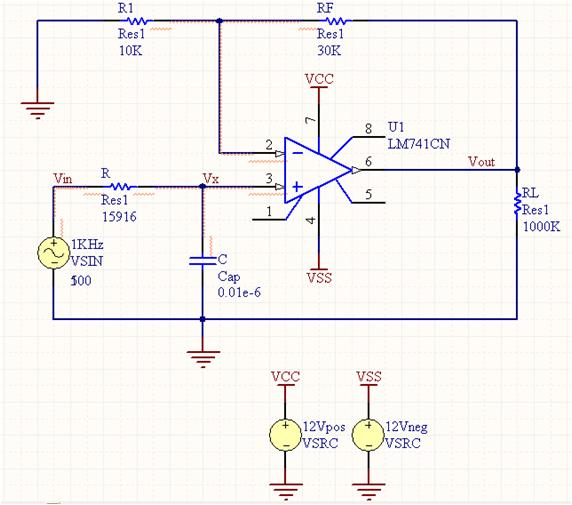
\includegraphics[width=4in]{FiltroPrimerOrdenpasabajas.jpg}
\caption{Filtro de primer orden}
\label{fig9}
\end{figure}

\section{El bicuadrático Sallen-Key}
La función bicuadrática, que sirve como bloque básico para una variedad de filtros activos, tiene la forma general 

\begin{equation}
H(s)=K \frac{k_2 s^2+k_1 (\omega_0/Q) s + k_0 \omega _0^2}{s^2+(\omega_0/Q) s+\omega_0^2}
\label{equ100}
\end{equation}
donde $\omega_0$ es la frecuencia natural no amortiguada (o de resonancia), $Q$ es el factor de calidad o cifra de mérito y $K$ es la ganacia de corriente directa. Las constantes $k_2$, $k_1$ y $k_0$ son $\pm 1$ o $0$. 
La rapidez de atenuación de un filtro de primer orden es de solo $-20 dB/década$ en la banda de atenuación. Un filtro de segundo orden tiene una reducción en la banda de atenuación de $-40 dB/década$ y, por tanto, se le prefiere en lugar de un filtro de primer orden. Además, el filtro de segundo orden se puede convertir en el bloque básico para construir filtro de mayor orden ($n=4,6,...$). Si se sustituye $k_2=k_1=0$ y $k_0=1$ en la ecuación general se obtiene

\begin{equation}
H(s)=\frac{K \omega_0^2}{s^2+(\frac{\omega _0}{Q}) s+\omega_0^2}
\label{equ101}
\end{equation}
donde $K$ es la ganancia en corriente directa. En la figura \ref{fig9} se muestra el esquemático de un bicuadrático Sallen-Key Modificado cuya función transferencia es

\begin{equation}
H(s)=\frac{\frac{K}{R_2 R_3 C_2 C_3}}{s^2+ s \frac{R_3 C_3+R_2 C_2+R_2 C_3}{R_2 R_3 C_2 C_3}+\frac{1}{R_2 R_3 C_2 C_3}}
\label{equ102}
\end{equation}

en donde $K=(1+ \frac{R_F}{R_1})$ es la ganancia de corriente directa. La ecuación \ref{equ102} es igual en forma a la ecuación \ref{equ101}. Haciendo el denominador igual a cero, se obtiene la ecuación característica

\begin{equation}
s^2+ s \frac{R_3 C_3+R_2 C_2+R_2 C_3}{R_2 R_3 C_2 C_3}+\frac{1}{R_2 R_3 C_2 C_3}=0
\label{equ103}
\end{equation}

\begin{figure}
\centering
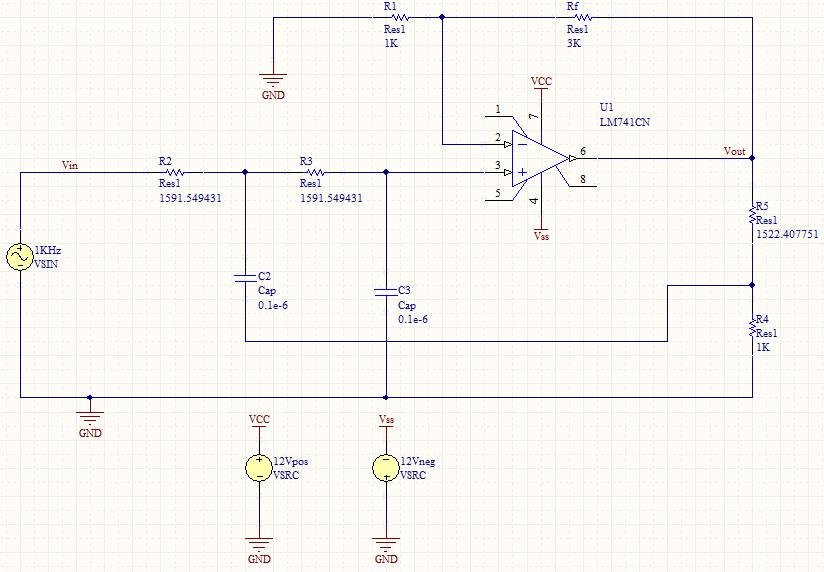
\includegraphics[width=4in]{BicuadraticoPasabajas.jpg}
\caption{Bicuadrático Sallen-Key modificado}
\label{fig10}
\end{figure}

Si comparamos en denominador de la ecuación \ref{equ101} con el denominador de la ecuación \ref{equ102} se puede concluir para el término independiente de $s$ que:

\begin{equation}
\omega _0 = \frac{1}{\sqrt{R_2 R_3 C_2 C_3}}
\label{equ104}
\end{equation}

Debido a la topología de amplificador no inversor de la figura \ref{fig9}, se considera que la ecuación de la ganancia es

\begin{equation}
K = 1+\frac{R_F}{R_1}
\label{equ105}
\end{equation}

Si consideramos que en la figura \ref{fig9} el divisor de voltaje en la salida se puede modelar por la ecuación:
\begin{equation}
x = \frac{R_4}{R_4+R_5}
\label{equ106}
\end{equation}
 entonces podemos sustituir las ecuaciones \ref{equ104}, \ref{equ105} y \ref{equ106} en la ecuación \ref{equ102} y obtenemos:

\begin{equation}
H(s) = \frac{K \omega _0^2}{s^2+(3-x K)\omega _0 s+\omega _0 ^2}
\label{equ107}
\end{equation}

y el factor de calidad $Q$ de la ecuación \ref{equ102} se obtiene despejando de \ref{equ107}

\begin{equation}
Q= \frac{1}{3-x K}
\label{equ108}
\end{equation}

\chapter{Aproximación de Filtro Butterworth }

La magnitud de una función de transferencia $|N(j\omega)|$ puede estar dada por una expresión matemática, un conjunto de valores, o una forma de onda. El objetivo de la aproximación consiste en obtener una función $F(s)$ tal que $|F(j\omega)|$ aproxima a la función $|N(j\omega)|$. Idealmente deseariamos que las dos funciones fuesen idénticas, lo que en muchos casos se puede lograr. Las especificaciones de magnitud se dan por lo general en la escala decimal o lineal o en la escala logarítmica. En este último caso las unidades usadas son los decibeles [ $20log|N(j\omega)|$ ], abreviados dB.

\section{Propiedades de la función $|N(j\omega)|$}
La función de magnitud debe satisfacer un conjunto de propiedades necesarias. Para comenzar nuestro estudio es más conveniente considerar el cuadrado de la función magnitud. De ésta manera podemos escribir

\begin{equation}
|N(j\omega)|^2=N(j\omega) N^*(j\omega)=N(j\omega) N(-j\omega)
\label{equ109}
\end{equation}

donde el asterisco indica el complejo conjugado. En esta ecuación estamos suponiendo que $N(s)$ es una función racional con coeficientes reales. En este caso, el complejo conjugado de $N(j\omega)$ se puede obtener sustituyendo  la variable por su conjugado, es decir, reemplazando $j$ por $-j$. La forma más general de $N(s)$ se puede escribir como

\begin{equation}
N(s) = \frac{c_0+c_1 s + c_2 s^2+ c_3 s^3+...}{d_0+d_1 s+d_2 s^2+d_3 s^3+...}
\label{equ110}
\end{equation}

De esta manera $N(j\omega)$ tendrá la forma

\begin{equation}
N(s) = \frac{c_0-c_2 \omega^2 + c_4 \omega^4-...+j(c_1 \omega - c_3\omega ^3+...)}{d_0-d_2 \omega ^2+d_4 \omega ^4-...+j(d_1 \omega - d_3 \omega ^3+...)}
\label{equ111}
\end{equation}

Sustituyendo la Ec. \ref{equ111} en el lado derecho de la Ec. \ref{equ109} obtenemos que $|N(j\omega)|^ 2$ es un cociente de polinomios pares. Esta es la primera propiedad que satisface $|N(j\omega)|$.

La función $|N(j\omega)|$ sólo es válida para el eje $j\omega$. De esta manera su utilidad es limitada. Podemos extender su validez a todo el plano s realizando una continuación analítica. Esto es equivalente a realizar un cambio de variable $\omega= s /j$. En este caso, $|N(j\omega)|$ se cambia a

\begin{equation}
|N(j\omega)| ^2_{\omega = \frac{s}{j}}= N(s) N(-s)
\label{equ112}
\end{equation}

En el lado derecho de la Ec.\ref{equ112}, el hacer el cambio de $s$ por $-s$ sólo refleja los polos y ceros de $N(s)$ sobre el eje imaginario. De esta manera, $N(s)N(-s)$ tendrá polos y ceros con simetría cuadrantal localizados simétricamente con respecto a los ejes real e imaginario. Esta es la segunda propiedad necesaria de una función de magnitud. En general, los polinomios del numerador y denominador de $N(s)N(-s)$ pueden tener tres tipos de factores:

\begin{enumerate}
\item $s^4+ a s^2+b$ donde $a$ y $b$ puede ser positivos o negativos
\item $a s^2+b$ donde $a$ y $b$ tienen signos opuestos
\item $a s^2+b$ donde $a$ y $b$ tienen el mismo signo
\end{enumerate}

Los dos primeros tienen la necesaria simetría cuadrantal, mientras que el tercero, que corresponde a ceros sobre el eje $j\omega$, sólo la tiene cuando aparece con multiplicidad par.

\subsection{Ejemplo: Función de circuito con polos y ceros con simetría cuadrantal}

\begin{equation*}
N(s) = \frac{s^2+1}{s^2+s+1}
\end{equation*}

Sustituyendo $j\omega$ por $s$, obtenemos

\begin{equation*}
N(j\omega)=\frac{1-\omega ^2}{1- \omega ^2+j\omega}
\end{equation*}

La magnitud está dada por

\begin{equation*}
|N(j\omega)|=\frac{(1-\omega ^2)^2}{(1-\omega ^2)+\omega ^2}=\frac{1-2 \omega ^2 + \omega ^4}{1- \omega ^2+ \omega ^4}
\end{equation*}

La cual sólo tiene potencias pares de$\omega$. Si formamos ahora $N(s)N(-s)$ tenemos que

\begin{equation*}
N(s) N(-s)= \frac{s^4+ 2 s^2+1}{s^4+s^2+1}
\end{equation*}

Tanto el numerador como el denominador tienen la simetría del primer tipo de factor posible.

La suficiencia de las dos propiedades se puede demostrar factorizando $N(s)N(-s)$ y asignando los polos que están en el semiplano izquierdo y la mitad de los ceros sobre el eje $j\omega$ a $N(s)$ y asignando los polos del semiplano derecho y los ceros restantes que están sobre el eje $j\omega$ a $N(-s)$. Los ceros se pueden asignar arbitrariamente. La restricción de usar sólo los polos del semiplano izquierdo es por razones de estabilidad.

	Usando las propiedades descritas es posible entonces obtener una función $N(s)$ a partir de la especificación de su magnitud.
	
\subsection{Ejemplo: Obtención de $N(s)$ a partir de su magnitud}

Consideremos la magnitud dada por

\begin{equation*}
|N(j\omega)|^2=\frac{\omega ^2+1}{\omega ^4 +1}
\end{equation*}

Sustiyendo $s/j$ por $\omega$ obtenemos que

\begin{equation*}
N(s) N(-s)=\frac{-s^2+1}{s^4+1}= \frac{(s+1)(-s+1)}{(s^2+\sqrt{2} s+1)(s^2-\sqrt{2}s+1)}
\end{equation*}

Asociando los polos en el semiplano izquierdo con $N(s)$, podemos formar dos funciones $N(s)$ que tienen la magnitud indicada y que además son estables. Estas funciones son

\begin{equation*}
N_1 (s)= \frac{s+1}{s^2+\sqrt{2} s+1}
\end{equation*}

y 
\begin{equation*}
N_2 (s)= \frac{s-1}{-s^2+\sqrt{2} s-1}
\end{equation*}

donde hemos invertido el signo en el numerador de $N_2 (s)$ ya que esto no afecta la magnitud.

\section{Funciones de magnitud máximamente plana}

Las propiedades obtenidas en la sección anterior para funciones de magnitud al cuadrado nos pueden servir para especificar características de filtros. Como nuestro primer caso, consideremos la determinación de una función cuya magnitud al cuadrado, para frecuencias bajas, tiene una característica tan plana como sea posible. Una manera de obtener esta característica es hacer tantas derivadas como sea posible iguales a cero en el punto $\omega= 0$. A esta función se le llama  función de magnitud máximamente plana. Para obtener dicha función haremos uso de la primera propiedad, es decir, que la magnitud al cuadrado es un cociente de polinomios pares:

\begin{equation}
|N(j\omega)| ^2 = H ^2 \frac{1+b_1 \omega ^2 + b_2 \omega^ 4+ b_3 \omega ^ 6 +...}{1+ a_1 \omega ^2+a_2 \omega ^4+a_3 \omega ^6+...}
\label{equ113}
\end{equation}

Realizando la división obtenemos

\begin{equation}
|N(j\omega)|^2= H^2 [1+(b_1-a_1)\omega ^2+ (b_2-a_2+a_1^2-a_1 b_1)\omega ^4+...]
\label{equ114}
\end{equation}

Consideremos ahora el desarrollo en serie de MacLaurin de la función $F(\omega)$

\begin{equation}
F(\omega)= F(0)+\frac{F^{(1)}(0)}{1!}\omega+\frac{F^{(2)}(0)}{2!}\omega ^2+\frac{F^{(3)}(0)}{3!}\omega ^3+...
\label{equ115}
\end{equation}

donde $F(i)$ es la iima derivada de $F(\omega)$ evaluada en $\omega= 0$. Comparando esta ecuación con la de $|N(j\omega)|^2$ dada en la Ec.\ref{equ114} y sabiendo que la expansión en serie es única, concluimos que todas las derivadas de orden impar tienen el valor de cero. Además, para que la segunda derivada sea cero se requiere que los coeficientes $a_1$ y $b_1$ sean iguales. De la misma manera, para que la cuarta derivada sea cero se requiere que $a_2$ sea igual a $b_2$, y así sucesivamente. En general, para que una magnitud al cuadrado sea máximamente plana se requiere que 

\begin{equation}
a_i=b_i
\label{equ116}
\end{equation}

para tantos coeficientes como sea posible.

\subsection{Ejemplo: Obtención de una función de magnitud máximamente plana}

Determínese la relación entre los coeficientes $a$, $b$ y $z$, para que $T(s)$ tenga magnitud máximamente plana para $T(s)$ dada por

\begin{equation*}
T(s)= \frac{s+z}{s^2+ as +b}
\end{equation*}

Para que $T(s)$ tenga magnitud máximamente plana lo primero es obtener y escribirla en la forma de la Ec.\ref{equ113}, con lo que obtenemos

\begin{equation*}
|T(j\omega)|^2 = \frac{z^2}{b^2} \frac{1+(\frac{1}{z^2})\omega ^2}{1+[(a^2-2 b)/b^2]\omega ^2+(1/b^2)\omega ^4}
\end{equation*}

Igualando los coeficientes de $\omega^2$ en el denominador y numerador, encontramos que la condición para magnitud máximamente plana es

\begin{equation*}
a^2-2 b =(\frac{b}{z})^2
\end{equation*}

\section{Filtros Butterworth}

Una de las funciones de magnitud más usadas es la función Butterworth, que recibe el nombre de su inventor. Consideremos una función pasabajos que tiene una característica plana para bajas frecuencias y cuyo valor cae a un valor pequeño para altas frecuencias. Un enfoque más práctico para realizar esta función de transferencia sería aproximar la magnitud ideal por una función que tenga una magnitud que satisfaga el criterio de magnitud máximamente plana en $\omega=0$. De esta manera se generaría la característica plana, al menos para bajas frecuencias. Además, para proporcionar la caida del valor de la magnitud para altas frecuencias, colocaremos todos los ceros en el infinito. De esta manera, El numerador de  $|N(j\omega)|^2$ sólo será una constante y los coeficientes $b_i$ serán todos iguales a cero. Para obtener la magnitud máximamente plana, los coeficientes $a_i$ también deben hacerse iguales a cero, excepto por el de mayor orden. La magnitud al cuadrado resultante tendrá entonces la forma

\begin{equation}
|N(j\omega)|^ 2 = \frac{H^2}{1+a_N \omega ^ {2 n}}
\label{equ117}
\end{equation}

El coeficiente $a_n$ por lo general se le denota por $\epsilon ^ 2$. De esta manera la Ec.\ref{equ117} se escribe como

\begin{equation}
|N(j\omega)|^ 2 = \frac{H^2}{1+\epsilon ^2 \omega ^ {2 n}}
\label{equ118}
\end{equation}

A esta función se la llama una función Butterworth.

Un análisis de esta función nos da las siguientes propiedades:

\begin{itemize}
\item El rango de frecuencias $0<\omega<1$ $rad/seg$ se llama \textbf{banda de paso}
\item El rango de frecuencias $\omega >1$ $rad/seg$ se llama \textbf{banda de rechazo}
\item Si sustituimos $\omega=1$ $rad/seg$ en la ecuaci\'{o}n \ref{equ118} obtenemos $|N(j\omega)|^ 2= \frac{H^2}{1+\epsilon ^2}$ independientemente del valor de $-n/2$
\item En $\omega = 1$ $rad/seg$, la pendiente de $|N(j\omega)|^2$ es proporcional a $-n/2$.
\item La función $|N(j\omega)|$ es una función monótonamente decreciente de $\omega$.
\end{itemize}

La ecuación definida por la ec. \ref{equ118} se llama \textbf{la Función Butterworth normalizada}.

\section{El parametro epsilon y la atenuación máxima}
Como se ha mencionada un filtro Butterworth es una función máximamente plana decreciente, lo cual implica, en el caso de filtros pasabajas, que la ganancia máxima se obtiene a las bajas frecuencias, y el punto en el cual la magnituda empezará a decaer es la frecuencia de corte. Al intervalo de frecuencia ente la frecuencia de corte y la frecuencia cero se le denomina banda de paso de tal forma que la banda de paso es el conjunto de frecuencias es las cuales no se desea que haya atenuación, sin embargo la atenuación es inevitable aunque  puede ser restringida a ciertos margenes de valor. Es por ello que a la atenuación en la banda de paso se le denomina \textbf{atenuación máxima}, la cual es la máxima caida en la magnitud en la banda de paso que se le permite al filtro.

\subsubsection{Obtención de la épsilon en base a la atenuación máxima}

Considerando la ecuación \ref{equ118} cuando la frecuencia es cero ($\omega=0$ obtenemos

\begin{equation}
|N(j0)|^ 2 = \frac{H^2}{1+\epsilon ^2 0 ^ {2 n}}= H^2
\label{equ120}
\end{equation}

Lo cual nos permite obtener:

\begin{equation*}
|N(j0)|= H
\end{equation*}

Si sustituimos la frecuencia de corte ($\omega _c =1$ para un filtro normalizado) en la ecuación \ref{equ118}

\begin{equation*}
|N(j1)|^2=\frac{H^2}{1+ \epsilon ^2 (1) ^{2n}}= \frac{H^2}{1+\epsilon^2}
\end{equation*}

de donde obtenemos:

\begin{equation}
N(j1)= \frac{H}{\sqrt{1+\epsilon ^2}}
\label{equ119}
\end{equation}

Si dividimos $|N(j0)|/|N(j1)|$ obtenemos

\begin{equation}
\frac{|N(j0)|}{|N(j1)|}= \sqrt{1+\epsilon ^2}
\label{equ121}
\end{equation}

Si a la ecuación \ref{equ121} la convertimos a decibeles entonces y le llamamos atenuación máxima 

\begin{equation}
A_{max}=20 \log \frac{|N(j0)|}{|N(j1)|}= 20 \log  \sqrt{1+\epsilon ^2}
\label{eq122}
\end{equation}

 De la ecuación \ref{equ121} despejamos $\epsilon$ y obtenemos

\begin{equation}
\epsilon = \sqrt{10 ^{\frac{A_{max}}{10}}-1}
\label{equ123}
\end{equation}

\section{Orden del filtro Butterworth}
La determinación del orden que debe tener una función Butterworth para satisfacer las especificaciones de atenuación se calcula utilizando la siguiente ecuación.

\begin{equation}
A_{min}= 20 \log \frac{|N(j0)|}{|N(j\omega _s)|}= 20 \log \sqrt{1+\epsilon ^2 \omega ^{2 n}}
\label{equ124}
\end{equation}

en donde la \textbf{atenuación mínima} $A_{min}$ es la mínima caída de la magnitud que se desea para el filtro Butterworth, y esta atenuación mínima se mide desde la frecuencia cero hasta el inicio de la banda de rechazo $\omega _s$.

Si despejamos $n$ de la ecuación \ref{equ124} obtenemos que

\begin{equation}
n > \frac{\log [\frac{10^{0.1 A_{min}}-1}{\epsilon ^2}]}{\log (\frac{\omega _s}{\omega _c})}
\label{equ125}
\end{equation}

\section{Polos de la función Butterworth}

Los polos de una función $N(s)$ con característica de magnitud Butterworth se obtiene a partir de la ecuación \ref{equ118} . De esta manera

\begin{equation}
N(s) N(-s) = \frac{H^2}{1+\epsilon ^2 (\frac{s}{j})^{2 n}}
\label{equ126}
\end{equation}

Haciendo el denominador de la ec. \ref{equ126} igual a cero, encontramos que los polos satisfacen la relación

\begin{equation}
s = \frac{1}{\sqrt[n]{\epsilon}}(-(-1)^n)^{\frac{1}{2 n}}
\label{equ127}
\end{equation}

De la ecuación \ref{equ127} si $n$ es par obtenemos

\begin{equation}
s = \frac{(-1)^{\frac{1}{2n}}}{\sqrt[n]{\epsilon}}= e^{\frac{(\frac{j \pi k} { 2n})}{\sqrt[n]{\epsilon}}}
\label{equ128}
\end{equation}

Para $k=1,3,5,... 4n-1$. De la ecuación \ref{equ127}, si $n$ es impar obtenemos

\begin{equation}
s = \frac{(1)^{\frac{1}{2n}}}{\sqrt[n]{\epsilon}}= e^{\frac{(\frac{j \pi k} { 2n})}{\sqrt[n]{\epsilon}}}
\label{equ129}
\end{equation}

Para $k=0,2,4,... 4n-2$. De las ecuaciones \ref{equ128} y \ref{equ129} vemos que los polos estan equidistantes y colocados sobre el círculo de radio $\frac{1}{\sqrt[n]{\epsilon}}$. Notese que los polos están espaciados un ángulo $\pi/n$. Por razones de estabilidad  sólo nos interesan los polos localizados en el semiplano izquierdo. Por lo tanto los polos de $N(s)$ están dados por $P_k=\sigma_k+j\beta _k$ donde

\begin{eqnarray}
\sigma_k = - \frac{1}{\sqrt[n]{\epsilon}} sen (\frac{2k-1}{2n}\pi) & \beta_k = - \frac{1}{\sqrt[n]{\epsilon}} cos (\frac{2k-1}{2n}\pi) & k = 1,2,3,...,n
\end{eqnarray}

Para cada polo complejo existe su complejo conjugado formando un par de polos complejos conjugados los que a su vez producen un factor cuadrático de la forma

\begin{equation}
s^2+ s \frac{2}{\sqrt[n]{\epsilon}} sen (\frac{2k-1}{2n}\pi)+(\frac{1}{\sqrt[n]{\epsilon}})^2
\label{equ130}
\end{equation}

Calculando la frecuencia y la calidad obtenemos

\begin{eqnarray}
\omega _k = \frac{1}{\sqrt[n]{\epsilon}} & Q_k = \frac{1}{2 sen (\frac{2k-1}{2n}\pi)} & k=1,2,...,n
\end{eqnarray}


\chapter{Filtro Chebyshev}

\section{Filtro Chebyshev Pasabanda}

Para obtener funciones de filtros pasabanda también se usa un filtro pasabajos al cual se le efectúa una transformación. 

\begin{figure}
\centering
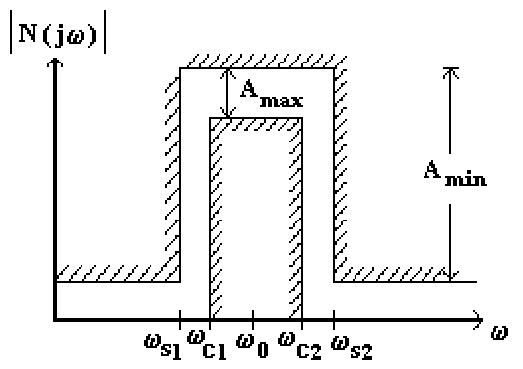
\includegraphics[width=3.5in]{PasabandaCheby.png}
\caption{Características de un filtro Pasabanda Chebyshev}
\label{fig11}
\end{figure}


Un filtro pasabanda tiene una banda de paso y dos bandas de rechazo como se muestra en la Fig \ref{fig11}. Las frecuencias que definen la banda de paso son
$\omega _{c1}$ y $\omega _{c2}$. Una de las bandas de rechazo empieza en c.d. y llega hasta la frecuencia $\omega _{s1}$ mientras que la otra banda de rechazo va de
$\omega _{s2}$ hasta el infinito. Dos parámetros que importantes de un filtro pasabanda son la frecuencia central $\omega _0$, el ancho de banda B y el factor de 
calidad Q. Estos parámetros están definidos por

\begin{equation}
 \omega _0 ^2 = \omega _{c1}\omega _{c2}
\label{equ300}
\end{equation}

\begin{equation}
 B = \omega _{c2}- \omega _{c1}
\label{equ301}
\end{equation}

\begin{equation}
 Q = \frac{\omega _{0}}{B}
\label{equ301}
\end{equation}

La ecuación \ref{equ300} indica que $\omega _0$ es la media geométrica de las frecuencias de la banda de paso. El factor de calidad Q indica que tan selectivo es 
el filtro. De las Ecs.(\ref{equ300}-\ref{equ301}) podemos calcular los valores de  $\omega _{c1}$ y $\omega _{c2}$ dados los valores de B y de $\omega _0$ con tan sólo resolver este sistema de ecuaciones, 
con lo que obtenemos

\begin{equation}
 \omega _{c1}= - \frac{B}{2}+\sqrt{\left(\frac{B}{2}\right)^2+\omega _0^2}
\label{equ302}
\end{equation}

\begin{equation}
 \omega _{c1}= \frac{B}{2}+\sqrt{\left(\frac{B}{2}\right)^2+\omega _0^2}
\label{equ303}
\end{equation}

Este resultado es válido para cualquier par de frecuencias que estén a ambos lados de la frecuencia central y que tengan a esta como media geométrica.

La transformación pasabajos a pasabanda  está definida por
\begin{equation}
 s= \frac{1}{B} \left(p+\frac{\omega _0^2}{p} \right)
\label{equ304}
\end{equation}

donde $s$ es la variable del filtro pasabajos y $p$ la variable del filtro pasabanda. $B$ será el ancho de banda del filtro pasabanda ( suponiendo que el filtro pasabajos
tiene ancho de banda normalizado) y $\omega _0$ será su frecuencia central.
Nótese que al igual que en el caso del filtro pasaaltos, la transformación pasabajos a pasaaltos se puede aplicar ya sea a la función de transferencia, 
a los polos y ceros o a los elementos del circuito pasabajos para obtener los elementos del filtro pasabanda.

Supongamos que deseamos convertir a pasabanda la función pasabajos 

\begin{equation}
 N_{pb}(s)=\frac{H}{a_0+a_1 s+a_2 s^2+...+a_{n-1}s^{n-1}+a_n s^n}
\label{equ305}
\end{equation}

Después de aplicar la transformación dada por la Ec.\ref{equ305} y multiplicar numerador y denominador por $p^n$ obtenemos

\begin{equation}
 N_{pb}(s)=\frac{H p^n}{b_0+b_1 p+b_2 p^2+...+b_{2n-1}p^{2n-1}+b_{2n} p^{2n}}
\label{equ306}
\end{equation}

La función pasabanda resultante tendrá un numerador cuyo único término será de grado $n$ y un denominador de grado $2n$, por lo tanto 
la función pasabanda será de orden $2n$, el doble del orden de la función pasabajos.

Si aplicamos la transformación pasabajos a pasabanda a los polos de la función pasabajos, los polos de la función pasabanda se pueden 
encontrar despejando la variable $p$ de la Ec.\ref{equ304} con lo que obtenemos

\begin{equation}
 p= \frac{s B}{2}\pm \sqrt{\left(\frac{s B}{2}\right)^2-\omega _0^2}
\label{equ307}
\end{equation}


\section{Bicuadrático Pasabanda de banda angosta}

\begin{figure}
\centering
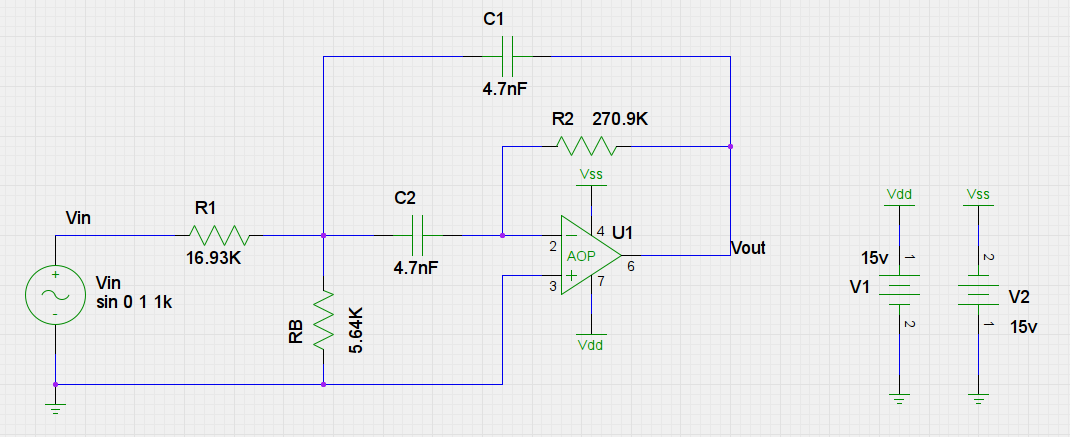
\includegraphics[width=3.5in]{BicuadPasabanda.png}
\caption{Filtro Bicuadrático Pasabanda de banda angosta}
\label{fig12}
\end{figure}

\subsection{Filtro Pasabanda de 40Khz para sensores ultrasónicos}


\backmatter
\end{document}
